\newpage
\section{Об эйлеровых и гамильтоновых циклах}

Теперь, будучи знакомыми с некоторыми терминами теории графов, мы можем более формально подойти к задаче, которую поставил в 1836 году Эйлер. И обобщить его теорию.

\mysubsection{Эйлеровы графы}

\begin{definition}
	Граф называется \emph{эйлеровым}, если в нём существует цикл, проходящий через все ребра ровно по одному разу. Если в графе есть эйлеров путь, то он называется \emph{полуэйлеровым}.
\end{definition}

\begin{lemma}[Лемма о простом цикле]
	В графе, состоящем только из чётных вершин, в котором есть хотя бы одна неизолированная вершина, есть простой цикл. 
	
	\emph{Доказательство.} Выберем вершину $A$~---~неизолированную вершину. Так как степень четна, то у $A$ есть, как минимум, два инцидентных ей ребра. Допустим, что одно из этих рёбер соединяет $A$ с вершиной $B$. Те же рассуждения верны и для $B$, поэтому есть вершина $C$, которая смежна $B$. И так далее. Так как у нас конечное число вершин, то в какой-то момент мы вернемся в какую-нибудь вершину, которую уже посещали. Если это будет не вершина $A$, то отбросим <<хвост>> и у нас останется простой цикл. ч.т.д.
\end{lemma}

\begin{theorem}[Критерий эйлеровости графа]
	Связный граф является эйлеровым тогда и только тогда, когда каждая его вершина имеет четную степень.
	
	\emph{Доказательство.} Из эйлеровости можно с легкостью вывести четность каждой вершины. Будем закрашивать ребра, проходя по эйлеровому циклу, тогда, проходя очередную вершину, мы закрасим два смежных с ней ребра. Следовательно, если какая-то вершина $s$ встречается $k$ раз в нашем эйлеровом цикле, то её степень равна $2k$: все ребра эйлерового цикла различны.
	
	Для того чтобы доказать обратное утверждение, опишем алгоритм нахождения эйлерового цикла. Для начала разобьем весь граф на простые циклы. Для этого, пользуясь леммой о простом цикле, будем выбирать простой цикл и стирать ребра, входящие в него. Так как в простом цикле у каждой вершины степень два, то четность вершин не будет меняться при таком алгоритме. В какой-то момент у нас все вершины станут изолированными, то есть фактически мы всё множество ребер разбили на непересекающиеся простые циклы.
	
	Назовем связанными те циклы, у которых есть хотя бы одна общая вершина. Заметим, что из связности графа следует связность выбранных простых циклов. Тогда покажем, как из двух связанных циклов сделать один цикл. Для этого рассмотрим вершину $s$, которая является общей для этих циклов. И сначала пройдем по одному циклу, а потом по другому. Таким образом мы обойдем все ребра обоих циклов ровно по одному разу и вернёмся в вершину, из которой стартовали. Таким образом, мы можем все циклы соединить в один цикл, который по построению будет содержать все ребра графа, то есть будет эйлеровым. ч.т.д.
\end{theorem}

\mysubsection{Гамильтоновы графы. Теорема Оре}

	Фактически эйлеров граф обязан своим появлением задаче о пути, проходящем через все рёбра. Аналогичная задача о пути, проходящем через все вершины, породила гамильтоновы графы.
	
\begin{definition}
	\emph{Гамильтонов путь (цикл)}~---~простой путь (цикл), проходящий через каждую вершину. Граф, в котором есть гамильтонов цикл, называется \emph{гамильтоновым графом}.
\end{definition}

	Впервые классы графов, в которых можно обойти все вершины, были введены ирландским математиком У. Гамильтоном (1805~---~1865) в 1856 году. В честь него они и были названы.
	
\begin{statement}
	Если в графе есть гамильтонов цикл, то в этом графе нет висячих и изолированных вершин.
	
	\emph{Доказательство.} У любой вершины произвольного цикла степень не меньше двух, а так как в гамильтонове графе через каждую вершину проходит гамильтонов цикл, то степень всех вершин не меньше двух. ч.т.д.
\end{statement}

	Наиболее известной задачей, связанной с гамильтоновыми графами, является задача коммивояжера: цель~---~пройти по всем городам страны за минимальное количество перемещений. Несмотря на очень схожее условие с задачей, поставленной Эйлером, для решения этой задачи не смогли ещё придумать оптимальный алгоритм, поэтому её всё ещё можно найти в списках $NP$-полных задач, куда она попала в $1972$ году, благодаря Ричарду Карпу.

	Гамилтоновы циклы нашли своё применение в теории шифрования, теории экстремальных задач. Кроме того, есть логические головоломки, в которых целью игры является поиск гамильтонова цикла с определёнными условиями.
	
	Аналогично задаче Эйлера, первый вопрос, который возникает при упоминании гамильтоновых циклов, связан с нахождением этого цикла в заданном графе. Кроме необходимого условия связности и условия на степени вершин, есть ещё следующее.
	
\begin{statement}
	Если в графе $G(V, E)$ есть гамильтонов цикл, то при удалении некоторого количества вершин $S \subset V$, количество компонент связности $k \colon= c(G-S)$ не превосходит числа удаленных вершин, то есть $k \leqslant |S|$.
	
	\emph{Доказательство.} Обозначим через $U_1, \dots, U_k$~---~компоненты связности, появившиеся после удаления множества вершин $S$ из графа. Тогда заметим, что в гамильтоновом цикле между вершинами двух разных компонент связности $U_i$ и $U_j$ обязательно будет вершина из множества $S$. Тогда можно поставить в соответствие каждой компоненте первую вершину из $S$, в которую мы попадаем по гамильтонову пути, выходя из соответствующей компоненты. Следовательно, по очевидному свойству вложения получаем искомое неравенство. ч.т.д.
\end{statement}

	На данный момент все известные необходимые условия не являются достаточными. Конечно, в некоторых графах очевидно гамильтонов цикл есть, например, в $C_n, n > 2$ и в $K_n, n > 2$.
	
	Предположим, что в графе есть гамильтонов путь. В каких графах мы его можешь достроить до цикла?
	
\begin{statement}
	Пусть в графе есть гамильтонов путь $P$, соединяющий вершины $x_1, x_n$, $n > 2$. Тогда для того чтобы в графе существовал гамильтонов цикл, достаточно $$deg(x_1)+deg(x_n) \geqslant n.$$
	
	\emph{Доказательство.} Во-первых, заметим, что если $x_1$ и $x_n$ смежны, то путь $P$ вместе с ребром $\lbrace x_n, x_1 \rbrace$ даёт гамильтонов цикл.
	
	Во-вторых, если это не так, то пусть степень вершины $x_1$ равна $k$, тогда если эти $k$ рёбер идут в вершины $x_{\alpha_1}, x_{\alpha_2}, \dots, x_{\alpha_k}$, то в одну из вершин $x_{\alpha_1 - 1}, x_{\alpha_2 - 1}, \dots, x_{\alpha_k - 1}$ ведёт ребро из $x_n$, так как иначе сумма $deg(x_1)+deg(x_n) \leqslant n$. Следовательно, допустим пара $x_m$, $x_{m+1}$ такова, что с $x_m$ соединена вершина $x_n$, а с $x_{m+1}$~---~$x_1$. Тогда искомый гамильтонов цикл~---~ $\langle x_1, x_2, \dots, x_m, x_n, x_{n-1}, \dots, x_{m+1}, x_1\rangle$. ч.т.д.
\end{statement}

\begin{consequence}
	Пусть в графе $G$ есть наибольший длины простой путь $P$, соединяющий вершины $x_1$, $x_n$. Тогда этот путь можно превратить в цикл $C$ либо в случае, если концы пути смежны, либо если сумма их степеней не меньше $n$.
\end{consequence}

	Так, как превращать гамильтонов путь в цикл, мы придумали. Теперь рассмотрим следующее достаточное условие существования гамильтонова пути.
	
\begin{theorem}[Оре]
	Если в графе $G(V, E), |V| = n > 2$ для любых двух вершин $a$ и $b$ выполняется неравенство 
	$$deg (a) + deg (b) \geqslant n-1,$$
	то в нём есть гамильтонов путь.
	
	\emph{Доказательство.} Фактически мы укажем путь, по которому можно построить гамильтонов путь. Заметим, что граф связен. Рассмотрим максимальной длины путь $P$. Если в нём $n$ вершин, то он гамильтонов. Иначе в силу утверждения выше мы можем превратить этот путь в цикл с таким же количеством вершин. С другой стороны,в этом цикле нет какой-то вершины графа, и так как он связен, то есть вершина, смежная с одной из вершин цикла. Тогда в графе есть путь большей длины, который начинается в этой вершине и обходит все вершины цикла. Противоречие. Следовательно, этот путь будет гамильтоновым.
\end{theorem}

\begin{consequence}
	Если в графе $G(V, E), |V| = n > 2$ для любых двух вершин $a$ и $b$ выполняется неравенство 
	$$deg (a) + deg (b) \geqslant n,$$
	то в нём есть гамильтонов цикл.
\end{consequence}

\begin{consequence}[Дирак]
	Если в графе $G(V, E), |V| = n > 2$ степень любой вершины не меньше $\frac{(n-1)}{2}$, то в нём есть гамильтонов путь. Если более того, неравенство верно для $\frac{n}{2}$ в правой части, то в графе есть гамильтонов цикл.
\end{consequence}

	Исторически так сложилось, что первым появилась теорема Дирака, доказанная им в $1952$ году. Далее пошёл шквал из всё более и более слабых условий на существование гамильтонова цикла. Утверждение, доказанное Оре, было тоже одним из этих <<порывов ветра>>. В $1972$ году Вацлав Хватал доказал теорему, охватившую все ранее известные достаточные условия. Однако в этом параграфе мы не будем её доказывать, а вернёмся позже к теореме Хватала.

	Эйлеровы циклы были созданы родоначальником теории графов и имели невероятный успех в своём освоении. К сожалению, гамильтоновы циклы, несмотря на столь же изящное определение, не могут порадовать читателей морем критериев и прочих интересных утверждений. Пока что гамильтоновы циклы остаются большой загадкой теории графов.

\mysubsection{Задачи}

\begin{exersize}
	Москвич Василий Петрович, приехавший в Санкт-Петербург поездом, весь день ходил по городу пешком. После столь утомительной прогулки он решил <<повысить градус>>. Посмотрев на карту, Василий Петрович заметил, что на всех улицах, по которым он проходил нечетное количество раз, расположены питейные заведения. Этот факт не мог не обрадовать москвича, так что было принято решение: вернуться на вокзал, проходя только по этим улицам. Докажите, что у Василия Петровича всё получится.
\end{exersize}

\begin{exersize}
	Мышка грызет куб сыра с ребром 3, разбитый на 27 единичных кубиков. Когда мышка съедает какой-либо кубик, она переходит к другому кубику, имеющему общую грань с предыдущим. Может ли мышка съесть весь куб, кроме центрального кубика?
\end{exersize}

\begin{exersize}
	При каких $n$ граф $K_n$ будет эйлеровым?
\end{exersize}

\begin{exersize}
	Какое минимальное количество отдельных проволок нужно, чтоб, не разрезая их, собрать каркас куба?
\end{exersize}

\begin{exersize}
	Верно ли, что можно на доске нарисовать произвольное количество касающихся окружностей, не отрывая мела? (если да, то докажите, что при произвольном расположении получится; если нет, то приведите контрпример)
\end{exersize}

\begin{exersize}
	В некоторой стране есть 2018 городов, соединенных подземными тоннелям, причём из любого города можно добраться до любого другого по подземным тоннелям, пройдя при этом все остальные города. Какое наименьшее число подземных тоннелей может быть в этой стране?
\end{exersize}
	
\begin{exersize}
	Верно ли, что в эйлеровом графе для любых двух смежных рёбер существует эйлеров цикл, в котором эти два ребра идут один за другим?
\end{exersize}

\begin{exersize}
	Докажите, что в эйлеровом графе нет мостов.
\end{exersize}

\begin{exersize}
	Подсчитайте количество гамильтоновых циклов в полном графе $K_n$, построенном на $n > 2$ вершинах.
\end{exersize}

\begin{exersize}[Канель-Белов А.Я., Ковальджи А.К. Как решают нестандартные задачи]
	Дан правильный $45$-угольник. Можно ли так расставить в его вершинах цифры от $0$ до $9$так, чтобы для любой пары различных цифр нашлась сторона, концы которой занумерованы этими цифрами.
\end{exersize}

\begin{exersize}[Генкин С.А., Итенберг И.В., Фомин Д.В. <<Ленинградские математические кружки>>]
	Доска имеет форму креста, который получается, если из квадратной доски $4 \times 4$ выкинуть угловые клетки. Можно ли обойти ее ходом шахматного коня и вернуться на исходное поле, побывав на всех полях ровно по разу?
\end{exersize}

\begin{exersize}[Канель-Белов А.Я., Ковальджи А.К. <<Как решают нестандартные задачи>>]
	В стране Метрополия каждый город связан с каждым дорогой. Злой волшебник установил на всех дорогах одностороннее движение. Тем не менее оказалось, что из любого города можно добраться до любого другого. Докажите, что существует замкнутый путь, проходящий через все города Метрополии один раз.
\end{exersize}

\begin{exersize}[Канель-Белов А.Я., Ковальджи А.К. Как решают нестандартные задачи]
	Последовательность из $36$ нулей и единиц начинается с пяти нулей. Среди пятерок подряд идущих цифр встречаются все $32$ возможные комбинации. Найдите пять последних цифр последовательности.	
\end{exersize}

\begin{exersize}[Бабичева Т.С., Бабичев С.Л., Жогов А. А., Яковлев И.В. <<Пособие по олимпиадной математике. Уровень А1>>]
	Можно ли нарисовать эту картинку, как на рисунке справа, не отрывая карандаша от бумаги и проходя по каждой линии по одному разу?
	
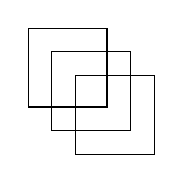
\begin{tikzpicture}
	\draw (0, 0) -- (-1, 0) -- (-1, -1) -- (0, -1) -- (0, 0);
	\draw (0.3, -0.3) -- (-0.7, -0.3) -- (-0.7, -1.3) -- (0.3, -1.3) -- (0.3, -0.3);
	\draw (0.6, -0.6) -- (-0.4, -0.6) -- (-0.4, -1.6) -- (0.6, -1.6) -- (0.6, -0.6);	
\end{tikzpicture}
\end{exersize}

\begin{exersize}[Бабичева Т.С., Бабичев С.Л., Жогов А. А., Яковлев И.В. <<Пособие по олимпиадной математике. Уровень А1>>]
	Существует ли эйлеров граф, из которого можно выделить эйлеров цикл несколькими различными способами?
\end{exersize}
